% 
% Annual Cognitive Science Conference
% Sample LaTeX Paper -- Proceedings Format
% 

% Original : Ashwin Ram (ashwin@cc.gatech.edu)       04/01/1994
% Modified : Johanna Moore (jmoore@cs.pitt.edu)      03/17/1995
% Modified : David Noelle (noelle@ucsd.edu)          03/15/1996
% Modified : Pat Langley (langley@cs.stanford.edu)   01/26/1997
% Latex2e corrections by Ramin Charles Nakisa        01/28/1997 
% Modified : Tina Eliassi-Rad (eliassi@cs.wisc.edu)  01/31/1998
% Modified : Trisha Yannuzzi (trisha@ircs.upenn.edu) 12/28/1999 (in process)
% Modified : Mary Ellen Foster (M.E.Foster@ed.ac.uk) 12/11/2000
% Modified : Ken Forbus                              01/23/2004
% Modified : Eli M. Silk (esilk@pitt.edu)            05/24/2005
% Modified : Niels Taatgen (taatgen@cmu.edu)         10/24/2006
% Modified : David Noelle (dnoelle@ucmerced.edu)     11/19/2014

%% Change "letterpaper" in the following line to "a4paper" if you must.

\documentclass[10pt,letterpaper]{article}

\usepackage{graphicx}
\usepackage{cogsci}
\usepackage{pslatex}
\usepackage{apacite}
\usepackage{gb4e}



\title{The Weakness of Epistemic \emph{must}}
 
\author{{\large \bf Gregory Scontras (scontras@stanford.edu), Judith Degen (jdegen@stanford.edu),}\\ {\large \bf Justine Kao (justinek@stanford.edu), Erin Bennett (erindb@stanford.edu),}\\ {\large \bf Noah D.~Goodman (ngoodman@stanford.edu)} \\
  Department of Psychology, Stanford University\\
  Stanford, CA 94305 USA}


\begin{document}

\maketitle


\begin{abstract}
We present results from three studies exploring the interpretation of statements featuring the epistemic necessity modal \emph{must}, comparing these statements to utterances with weaker modals, or no modals at all. Our results demonstrate that \emph{must}-statements coincide with less certain belief states, such that ``It must be raining'' receives a weaker interpretation than bare ``It is raining.'' Rather than engineering weakness into the meaning of the word \emph{must}, our account derives its weakness as an M-implicature \cite{levinson2000}. Statements with \emph{must} are marked relative to bare statements, so they communicate a marked meaning, namely less certainty on the part of the speaker. A general model of rational inference in communication delivers the puzzlingly weak interpretation of \emph{must}.
	
\textbf{Keywords:} 
pragmatics; semantics; psycholinguistics; modals; M-implicature 
\end{abstract}


\section{Introduction}

Modals come in varying degrees of strength; the strongest are modals of necessity like \emph{must} or \emph{have to}. Under a quantificational treatment of modality, these necessity modals correspond to universal quantifiers over possible words (XXX citation). When used, they assert that in every (relevant) possible world, some proposition \emph{p} holds. In (\ref{must}), epistemic \emph{must} is used to assert that in every world compatible with the speaker's knowledge, it is raining. Given that knowledge corresponds to justified true belief (that which is known cannot be otherwise), from (\ref{must}) it necessarily follows that it is raining (i.e., it is not possible that it is not raining). There are other analyses of modals on the market (e.g., a scalar semantics for modals; \citeNP{lassiter2011}), but all of them share the intuitive understanding of necessity modals as maximally strong semantic objects. 

\begin{exe}
	\ex\label{inference} \begin{xlist}
		\ex\label{might} It might be raining.
		\ex\label{must} It must be raining. 
		\ex\label{bare} It is raining.
	\end{xlist}
\end{exe}

When compared with other modals, necessity modals do behave as strong: (\ref{must}) expresses a stronger statement about rain than (\ref{might}). However, when compared to the bare statement without a modal, \emph{must} and other epistemic necessity modals suddenly behave as weak, or so the liturgy goes.  At issue is the failed inference from (\ref{must}) to (\ref{bare}) first observed by \citeA{karttunen1972}: How could \emph{must p} not entail \emph{p}? If it is necessarily raining, then surely it is raining. It appears that talking about what is necessarily the case commits speakers to less than does talking about what is actually the case. \citeauthor{karttunen1972} and decades of semanticists that followed posit that the inference from (\ref{must}) to (\ref{bare}) fails because \emph{must p} is a weaker statement than bare \emph{p}. In other words, \emph{must} is weak. Our first task is to evaluate the relative strength of \emph{must}, an empirical investigation conspicuously absent from the discussion of this modal thus far. Having justified the strength of \emph{must} empirically, we may then set our sights on the proposals meant to account for \emph{must}'s meaning.

Linguists split on the semantics of \emph{must}. The original ``\emph{must} is weak'' mantra, stemming from \citeA{karttunen1972}, has \emph{must p} not entail \emph{p}. There are two tacks to breaking this entailment. For \citeA{kratzer1991}, the entailment fails because  \emph{must p} is weaker than we might have thought. She weakens \emph{must} by having it quantify not just over knowledge states, but also over expectations given knowledge states -- expectations which are not always borne out. For \citeA{veltman1985}, the entailment fails because bare \emph{p} is stronger than we might have thought. He strengthens bare \emph{p} by allowing partial knowledge states, such that \emph{must p} may be true while we lack the knowledge to say whether \emph{p} is true or false. Either way, from \emph{must p} (e.g., ``It must be raining'') it does not follow that \emph{p} (e.g., ``It is raining'').

\citeA{vonfintelgillies2010} lead the opposing charge, holding firm to the logic that \emph{must p} is strong, quantifying universally over epistemically possible worlds. In addition to this strong semantics, they also claim that \emph{must} is an evidential marker, presupposing that the speaker has no direct evidence of \emph{p}. However, the strength of \emph{must p} requires the speaker to have direct evidence of something that entails \emph{p}. Using a corpus of naturally-occurring examples from Ancestry.com, \citeauthor{lassiter2014salt} (\emph{to appear}) shows how \citeauthor{vonfintelgillies2010}'s implementation of a strong semantics for \emph{must} makes unreasonable claims about the knowledge states of speakers. \citeauthor{lassiter2014salt} proposes instead a weak probabilistic semantics: \emph{must p} entails that the probability of \emph{p} given the speaker's direct knowledge is greater than chance, and requires that the question of whether \emph{p} not be resolved by this direct knowledge. Thus, he returns to the original mantra of weakness while building evidential information into the semantics of \emph{must}.

In an effort to inform this debate on the strength of \emph{must}, we first investigate what gets communicated via its use. Over the course of three experiments, we asses the speaker commitments, evidence strength, and listener understanding that accompany \emph{must} statements. Our findings qualitatively confirm \citeauthor{karttunen1972}'s original observation, and quantitatively demonstrate the relative weakness of \emph{must}. Moreover, they highlight the role of evidence strength in the computation of \emph{must}'s meaning -- an ingredient that has thus far been lacking from the proposed semantics for \emph{must}.

We then use our findings to motivate a computational model of the meaning of \emph{must}, following \citeA{lassitergoodman2013} in their extension of the Bayesian Rational Speech Act framework \cite{frankgoodman2012}. Rather than engineering weakness relative to bare \emph{p} directly into the meaning of the word \emph{must}, our account derives its weakness as an M-implicature \cite{levinson2000}: \emph{must p} is marked (i.e., costly) relative to the bare form (\ref{bare}); the bare form is sufficiently strong already to convey \emph{p} (e.g., that it is raining), so listeners take the marked form to convey the marked meaning that the speaker arrived at the conclusion \emph{p} via an evidentially less certain route than if they had chosen the shorter, bare form. Our account accomplishes two things. First, it obviates the conceptual pitfalls of \citeauthor{vonfintelgillies2010}'s strong semantics, without treating \emph{must} as inherently weak: evidence strength is inferred from, rather than communicated by, the use of \emph{must}. Second, it implements a formal model of M-implicatures within the Rational Speech Act framework \cite{bergenetal2014}.

%Our approach incorporates elements from both \citeA{vonfintelgillies2010} and \citeauthor{lassiter2014salt} \emph{to appear}: \emph{Must} is strong, but reasoning about its strong meaning yields a weaker interpretation.


\section{Experiment 1: Evidence}

Most discussions of \emph{must} make claims about the quality and/or quantity of evidence involved in its assertion. To better understand the meaning of \emph{must}, we therefore began by collecting estimates of evidence strength. These estimates were used in the analyses of Experiments 2 and 3, which target \emph{must}'s meaning directly.

\subsection{Participants, materials, and methods}

40 participants were recruited through Amazon's Mechanical Turk crowd-sourcing service, and were compensated for their participation.

Subjects rated the probability of some state of affairs \emph{p} (e.g., ``It is raining'') given a piece of evidence (e.g., ``You hear the sound of water dripping on the roof'') on a sliding scale with endpoints labeled ``impossible'' and ``absolutely certain''. There were four difference states (rain, cold coffee, dinner ready, dog barking), and for each state subjects evaluated one of five possible pieces of evidence.

\subsection{Results and discussion}

Probability ratings were averaged across subjects for each state of affairs and evidence type, and ranged from XX to XX, with a standard deviation of XX. These average ratings serve as a measure of evidence strength: higher probability ratings signal greater strength of evidence. We used these ratings in the design and analyses of Experiments 2 and 3.

\section{Experiment 2: Speakers}

Next, we evaluated the intuitions of speakers in a forced production task, testing how likely they are to use \emph{must p} vs.~bare \emph{p} as evidence strength decreases. In other words, we tested the relationship between \emph{must} and the evidence justifying its use.

\subsection{Participants, materials, and methods}

We recruited 40 participants from Amazon's Mechanical Turk. Participants were compensated with a small payment.

On each trial, participants were presented with a piece of evidence (e.g., ``You see a person come in from outside with wet hair and wet clothes'') and were asked to choose one of three possible utterances to describe a state of affairs \emph{p} to a friend given the available evidence. We used the same pieces of evidence and states of affairs from Experiment 1. For example, in describing the rain state, speakers chose between the three utterances in \ref{rain}.

\begin{exe}
	\ex\label{rain} \begin{xlist}
		\ex It might be raining. \hfill (\emph{might})
		\ex It must be raining. \hfill (\emph{must})
		\ex It is raining. \hfill (\emph{bare})
		\end{xlist}
		\end{exe}
		
\noindent Speakers completed four trials, one for each of the possible states.		

\subsection{Results and discussion}

Fig.~\ref{expt2} plots selection rates for the \emph{might}, \emph{must}, and \emph{bare} utterances against the evidence strength estimates from Experiment 1. Participants were more likely to choose the more marked \emph{must} form over the bare form as evidence strength decreased ($\beta$=5.4, \emph{SE}=2.4, \emph{p}$<$0.05). 

\begin{figure}
\centering
{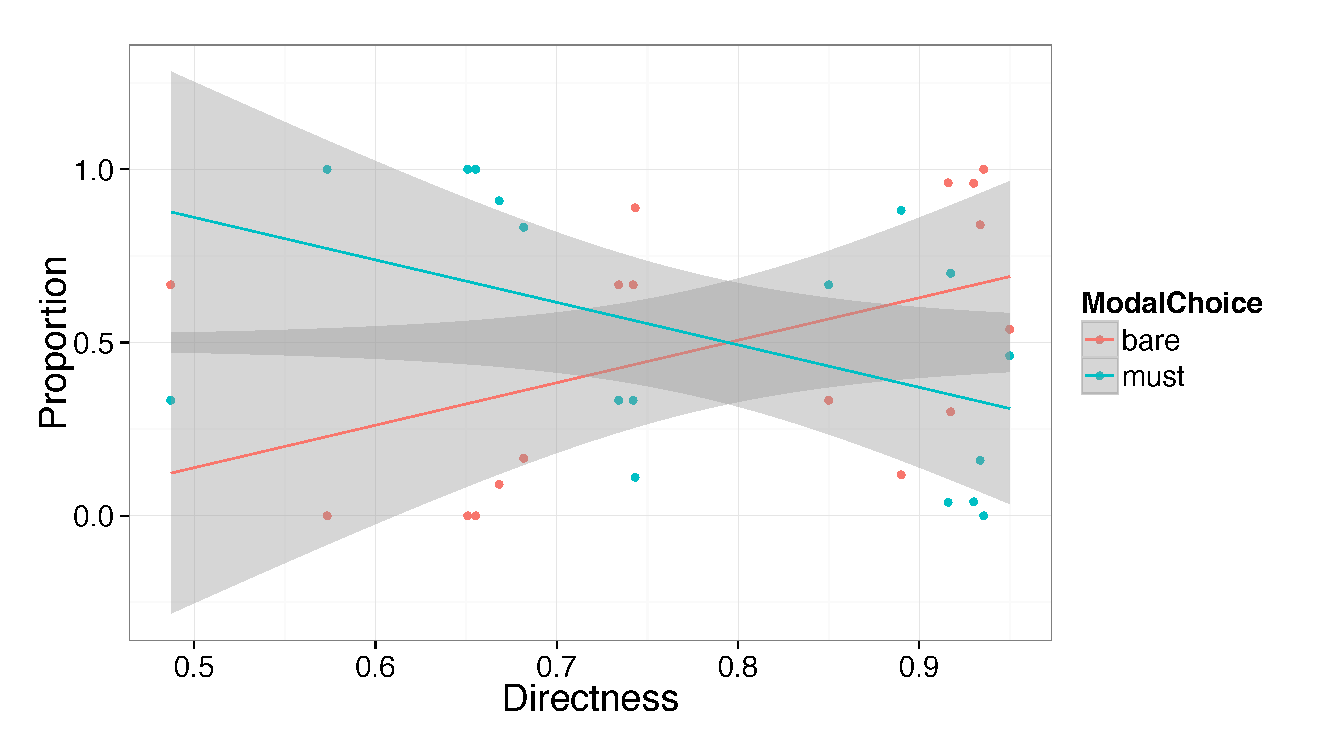
\includegraphics[width=\linewidth]{expt2.eps}}
\caption{Utterance choice plotted against evidence strength (Expt.~2).}
\label{expt2}
\end{figure}


\section{Experiment 3: Listeners}

Having found that speakers' use of \emph{must} increases as evidence strength decreases, we next tested whether listeners take into account this information about speakers as they interpret the bare and \emph{must} forms. In testing listeners' interpretation of \emph{must}, we also evaluated its relative strength.

\subsection{Participants, materials, methods}

We recruited 120 participants through Amazon's Mechanical Turk. Participants were compensated with a small payment.

We used the same four states of affairs and pieces of evidence from Experiments 1 and 2. On each trial, participants were presented with an utterance (e.g., ``It must be raining'') and asked a) to rate the probability of the state of affairs \emph{p} (e.g., of rain) on a sliding scale with endpoints labeled ``impossible'' and ``certain''; and b) to select one out of five pieces of evidence that the speaker had about \emph{p} in making their utterance.

\subsection{Results and discussion}

Fig.~\ref{expt3a} plots listener belief given utterance: participants believed \emph{p} was less likely after observing the \emph{must} utterance than after observing the \emph{bare} utterance ($\beta$=-0.21, \emph{SE}=0.01, \emph{t}=-10.1, \emph{p}$<$0.0001). Fig.~\ref{expt3b} plots average strength of evidence assumed for each utterance. Average evidence strength was lower for \emph{must} than for the bare utterance ($\beta$=-0.08, \emph{SE}=0.01, \emph{t}=-6.8, \emph{p}$<$0.0001).

\begin{figure}
	\centering
	{\includegraphics[width=\linewidth]{expt3a.eps}}
	\caption{Listener beliefs about the state of affairs \emph{p} after hearing a given utterance (Expt.~3).}
	\label{expt3a}
\end{figure}

\begin{figure}
	\centering
	{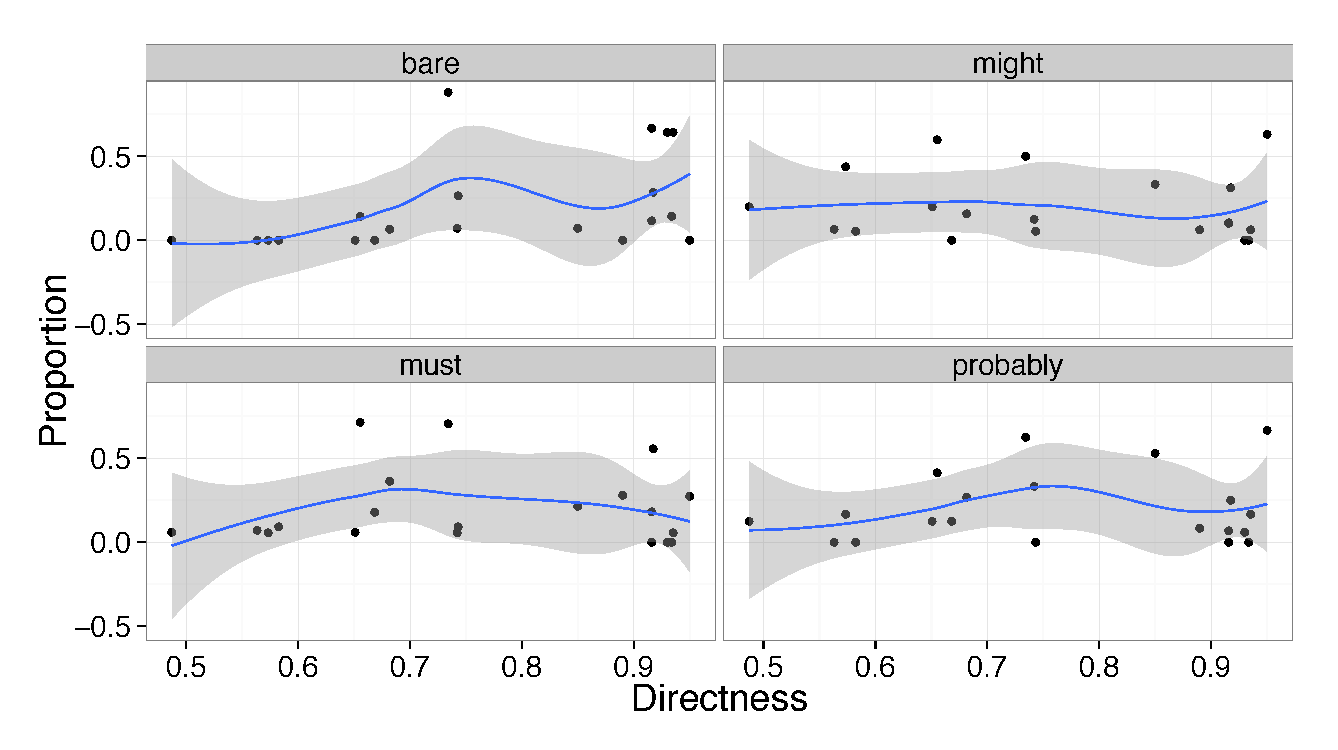
\includegraphics[width=\linewidth]{expt3b.eps}}
	\caption{Assumed evidence strength for a given utterance (Expt.~3).}
	\label{expt3b}
\end{figure}




\section{Model}

We propose a computational model of language understanding to show that the empirically verified, relatively weak interpretation of \textit{must} does not require encoding weakness or indirectness into the semantics of modals, but can  arise instead from pragmatic reasoning about its strength. In fact, already in \citeA[pp.~33--34]{grice1989} do we find inspiration for the calculation that leads to the relative weakness of \emph{must}:

\begin{quotation}
	``A wants to know whether \emph{p}, and B volunteers not only the information that \emph{p}, but information to the effect that it is certain that \emph{p}\ldots\ B's volubility may be undesigned, and if it is so regarded by A it may raise in A's mind a doubt as to whether B is as certain as he says he is\ldots\ But if it is thought of as designed, it would be an oblique way of conveying that it is to some degree controversial whether or not \emph{p}.''
\end{quotation}

\noindent Here, we formalize \citeauthor{grice1989}'s description of the computation. 

Our model follows the basic structure of Rational Speech Act (RSA) models, which view language understanding as recursive reasoning between speaker and listener \cite{frankgoodman2012}.

\section{Conclusion}





\section{Acknowledgments}



\bibliographystyle{apacite}

\setlength{\bibleftmargin}{.125in}
\setlength{\bibindent}{-\bibleftmargin}

\bibliography{greg}


\end{document}
